\documentclass[nopreprintline,12pt]{elsarticle}
%\setcounter{secnumdepth}{1} %auf 0, wenn Sections nicht nummeriert werden sollen

\usepackage{fancyhdr}


\pagestyle{fancy}
\fancyhf{}
%\renewcommand{\sectionmark}[1]{ \markright{#1} }
\thispagestyle{empty}
\fancyhead[R]{\rightmark}
\fancyhead[L]{}
\fancyfoot[C]{\thepage}

\usepackage{todonotes} %für Markierungen
%\usepackage[disable]{todonotes} um alle gleichzeitig wegzukriegen

\fancypagestyle{frontmatter}   % für seiten mit chapter titel
{
  \fancyhf{}
  \fancyhead[R]{\rightmark}
  %\fancyhead[L]{\leftmark}
  %\lhead{}
  %\rhead{\leftmark}
  \fancyfoot[C]{\thepage}
}

\fancypagestyle{mainmatter}   % für seiten mit chapter titel
{
  \fancyhf{}
  \fancyhead[R]{\rightmark}
  %\fancyhead[L]{\leftmark}
  %\lhead{}
  %\rhead{\leftmark}
  \fancyfoot[C]{\thepage}
}

\renewcommand{\headrulewidth}{0.5pt}

\renewcommand{\chaptermark}[1]{%
\markboth{\thechapter. \ #1}{}}

\usepackage{newtxtext,newtxmath}

\usepackage{lipsum,graphicx,float}
\usepackage{caption}
%\usepackage{subcaption}
\usepackage{subfig}
%\usepackage{float}

\usepackage{amssymb}

\usepackage{lineno}

\usepackage{xcolor} %Text in Farbe

\usepackage[ngerman]{babel} %Deutsch
\usepackage[utf8]{inputenc}

\usepackage[onehalfspacing]{setspace} %Zeilenabstand

\usepackage[toc,page]{appendix}

%\makeatletter
%\def\ps@pprintTitle{%
%   \let\@oddhead\@empty
%   \let\@evenhead\@empty
%   \let\@oddfoot\@empty
%   \let\@evenfoot\@oddfoot
%}
%\makeatother

\setlength{\headheight}{15pt}


%% `Elsevier LaTeX' style
\usepackage{natbib}
\usepackage{apalike}
\bibliographystyle{apalike}
%%%%%%%%%%%%%%%%%%%%%%%
\author{Cristina Ballero Reque}
\title{Einfluss von Schlaf auf die Gedächtnisleistung}
\address{Ruhr-Universität Bochum}
\address{Arbeitseinheit Neuropsychologie}
\journal{Dr. Lorena Deuker}


\begin{document}

%\maketitle
%\pagenumbering{gobble}
%% Title, authors and addresses


\begin{frontmatter}
\begin{abstract}
    xkml
\end{abstract}
\begin{keyword}
Science \sep Publication \sep Complicated
\end{keyword}
\end{frontmatter}


%%%%%%%%%%%%%%%%%%%%%%%
%% Elsevier bibliography styles
%%%%%%%%%%%%%%%%%%%%%%%
%% To change the style, put a % in front of the second line of the current style and
%% remove the % from the second line of the style you would like to use.
%%%%%%%%%%%%%%%%%%%%%%%


%% APA style
%\bibliographystyle{model5-names}\biboptions{authoryear}

\newpage

\pagenumbering{gobble}

\newpage


\pagenumbering{gobble}
\tableofcontents
\clearpage
\pagenumbering{arabic}

\section{Einleitung}
\label{S:1}


\paragraph{Unterteilung KZG/LZG}
Grundlagentext moodle
Deklarativ/nicht deklarativ
Gedächtnisbildung 3 Phasen

\paragraph{Gedächtnis(konsolodierung) und Schlaf}
Review Rasch \& Born
--> Unterteilung in Schlaf-/Taggruppe
Vorteile von Schlaf auf (wenn möglich) implizites (prozedural) Lernen

evtl. Studie zu Mittagsschlaf (sonst in Diskussion als post-hoc)

\paragraph{implizites Lernen Verhalten/EEG}
Bacchus-Studie (zeitliches Lernen)
Assoziation von Stimuli

\paragraph{Gavert-Studie mit Graphenstruktur}

\section{Methoden}
\label{S:2}

\subsection{Stichprobe}
Die Erhebung erstreckte sich über einen vierwöchigen Zeitraum von Ende April bis Mitte Mai 2018. Dabei nahmen insgesamt 52 Versuchspersonen an der Studie teil. Aufgrund einer Änderung der  EU-weiten Datenschutzrichtlinien wurden keine soziodemographischen Daten erhoben. Voraussetzung für die Teilnahme an der Studie waren ein Mindestalter von 18 Jahren, eine ausreichende (evtl. korrigierte) Sehkraft. Um Beeinträchtigungen der Erinnerungsleistung zu minimieren, wurden die ProbandInnen außerdem angewiesen, unmittelbar vor der Testung sowie in den darauffolgenden zwölf Stunden keinen Alkohol zu konsumieren. Außerdem wurden Personen ausgeschlossen, die an Epilepsie erkrankt sind.
Die Studie wurde im Rahmen eines universitären Seminars durchgeführt, bei dem mehrere Studierende zusammenarbeiteten. Die Rekrutierung der Studienteilnehmer wurde daher auf die Beteiligten aufgeteilt. Jeder Studierende sollte nach Möglichkeit vier Personen in seinem privaten Umfeld für die Studie anwerben und testen. Es gab keine Vergütung für die Teilnahme an der Studie.

\subsection{Versuchsdesign}
Zur Überprüfung der Hypothesen und zur Vermeidung von Lern-Effekten wurde ein Between-Subject Versuchsdesign gewählt. Dazu wurden die ProbandInnen im Vorhinein zufällig einer von zwei Gruppen zugeteilt, die als „Schlafgruppe“ (n = 25) und „Taggruppe“ (n = 27) benannt wurden. Die beiden Gruppen unterschieden sich hinsichtlich der Zeitpunkte, zu denen die zweiteilige Studie durchgeführt wurde. ProbandInnen der Schlafgruppe führten den ersten Teil abends durch und absolvierten den folgenden Teil am darauffolgenden Morgen. Bei der Taggruppe fand die Testung im Laufe eines Tages statt; morgens wurde der erste, abends der zweite Teil bearbeitet. Wichtig dabei war die Einhaltung eines zwölfstündigen Zeitraums zwischen beiden Testungen.

\subsection{Versuchsaufbau}
Die Studie wurde mittels des Simulationsprogramms \textit{Matlab\_R2018a} an den Computern der Studierenden durchgeführt. Die verwendeten Stimuli waren im Vorhinein von der Arbeitseinheit für Neuropsychologie in einem 3D-Programm  erstellt worden. Es \textcolor{purple}{handelt} sich dabei um fiktive Objekte in Grautönen, die möglichst keine Ähnlichkeit zu Alltagsgegenständen haben sollten. Dies wurde mittels eines Fragebogens abgesichert, den die Seminarteilnehmenden vor Beginn der eigentlichen Testung ausfüllten. Die angegebenen Assoziationen der Stimuli zu Alltagsgegenständen führten zum Ausschluss von zweien der ursprünglich 20 Stimuli.
Aus den verbleibenden 18 Stimuli wurden drei gleich große Gruppen gebildet, die als \textit{Communities} bezeichnet wurden. Dabei war die Zuordnung von jeweils sechs Stimuli zu einer Community für jede Versuchsperson randomisiert.
Darüberhinaus gab es von jedem Stimulus eine Standardversion und eine Version in rotierter Ausrichtung. Letztere wurde von einem Teil der Studierenden erstellt und nahm später die Funktion eines Distraktors ein \textcolor{purple}{(für Beispiele für Stimuli s. Untenstehende Graphik}.
\todo{HIER DAS PARADIGMA = GRAPHENSTRUKTUR EINBAUEN? JA!}


\begin{figure}[h]
\begin{subfigure}{0.5\textwidth}
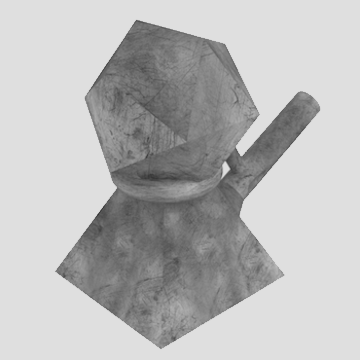
\includegraphics[width=0.9\linewidth, height=5cm]{Bilder/Objekt11A.png}
\caption{Original}
\label{fig:subim1}
\end{subfigure}
\begin{subfigure}{0.5\textwidth}
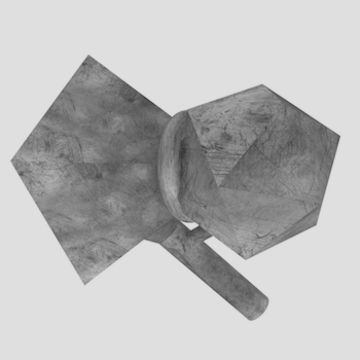
\includegraphics[width=0.9\linewidth, height=5cm]{Bilder/Objekt11B.png}
\caption{Rotiert}
\label{fig:subim2}
\end{subfigure}

\caption{Beispielhafter Stimulus in zwei Ausrichtungen}
\label{fig:image2}
\end{figure}

\subsection{Versuchsablauf}
Das Experiment war in zwei Teile unterteilt, die von allen Studienteilnehmenden in gleicher Reihenfolge absolviert wurden.

\paragraph{Encoding} Im ersten Teil, dem \textit{Encoding} sollten die ProbandInnen mit den Stimuli vertraut gemacht werden. Dazu wurden Sequenzen der Stimuli mit einer Target-Detektions-Aufgabe verbunden. Zu Beginn gab es nach einer Instruktion durch die Versuchsdurchführenden 20 Trials zur Übung, bei denen vor einem weißen Hintergrund \textcolor{purple}{in 5\% der Fälle} ein Distraktor (ein graues Rechteck) erschien, das mittels Tastendruck detektiert werden sollte. \textcolor{purple}{Zu langer Satz?}

Daraufhin begann die eigentliche Aufgabe mit insgesamt 720 Trials, die in sechs gleich großen Blöcken (à 120 Trials) gezeigt wurden. Bei den ersten drei Durchgängen sollten die Versuchsteilnehmenden den Distraktor wie zuvor in Form eines grauen Rechtecks \textcolor{purple}{(redundant?)} identifizieren. In den folgenden Durchgängen fungierten die Objekte in rotierter Version als Distraktor. Die Häufigkeit, mit der die zu identifizierenden Targets erschienen, war zuvor von den Versuchsdurchführenden festgelegt worden: das graue Kästchen tauchte in 5\% der Fälle auf, die rotierten Objekte in 15\%. Durch die geringe Auftretenswahrscheinlichkeit sollte eine stabil hohe Konzentration der ProbandInnen gewährleistet werden. Diese wurde als Voraussetzung zum impliziten Erlernen der Graphenstruktur gesehen.
Während der Trials wurden die Stimuli jeweils für eine Sekunde dargeboten, wonach sie verblassten und nach ebenfalls einer Sekunde der nächste Stimulus auftauchte. Zwischen jedem Block gab es eine Pause, in der neun Landschaftsbilder für jeweils zehn Sekunden dargeboten wurden. Die Landschaftsbilder wurden bei der Versuchsplanung von der Seminarleitung ausgewählt und sollten der Entspannung zwischen den einzelnen Durchgängen dienen. Außerdem wurde nach dem dritten Block (am Ende der Pause) der Wechsel des Distraktorentyps angekündigt. Insgesamt betrug damit die Dauer des ersten Teils etwa 35 Minuten.

\paragraph{Retrieval} Der zweite Teil der Studie, das \textit{Retrieval} war in zwei verschiedene Aufgaben unterteilt, die im Vergleich zum Encoding-Teil eine kürzere Bearbeitungszeit hatten. Daher wurden die Instruktionen für beide Aufgaben gleichzeitig gegeben.

Bei der ersten Aufgabe des Retrievals, \textit{odd one out}, wurden zu Beginn in acht Übungsdurchgängen jeweils drei Landschaftsbilder nebeneinander angeordnet gezeigt. Unter den drei Bildern sollten die ProbandInnen diejenige Landschaft auswählen, die ihrem subjektiven, intuiven Eindruck nach nicht dazugehört. Dazu konnte innerhalb eines bestimmten Zeitfensters (2.5 s) eine von drei Tasten gedrückt werden, die jeweils einer Position der Bilder entsprach (links, mittig, rechts). Ein Pausieren während dieser siebenminütigen Aufgabe war nicht möglich. Bei einer Reaktion außerhalb des vorgegebenen Zeitfensters erschien ein Hinweis auf dem Display mit der Bitte um schnellere Antwort. Nachdem die Teilnehmenden die Zuordnung der Tasten gelernt und sich an das Antwortzeitlimit gewöhnt hatten, wurden anstelle der Landschaftsbilder die eigentlichen Stimuli angezeigt. Die drei angezeigten Stimuli, auch \textit{Triplet} genannt, stammten aus verschiedenen Kategorien. Sie unterschieden sich bezüglich ihrer Distanz und Community-Zuordnung auf der zugrundeliegenden Graphenstruktur. Vor Versuchsbeginn waren acht verschiedene Kategorien identifiziert worden, aus denen jeweils maximal 18 Triplets präsentiert werden sollten. Welcher Stimulus dabei an welcher Position präsentiert wurde, wurde randomisiert. Zusätzlich wurden für die spätere Auswertung im Vorhinein pro Kategorie diejenigen Stimuli identifiziert, die aufgrund der Graphenstruktur (nicht) ausgewählt werden sollten.\textcolor{purple}{Näher ausführen?}

Aufgabe der zweiten Retrieval-Aufgabe, \textit{Sorting}, war es, die Stimuli zu sortieren. Ohne eine konkrete Zeitvorgabe sollten die Teilnehmenden dabei die kreisförmig angeordneten Objekte durch drag and drop anordnen. Für die Einteilung wurden wie bei der vorigen Aufgabe keine konkreten Kriterien gegeben; die ProbandInnen sollten auch dann eine Entscheidung treffen, wenn sie keine Regeln zu erkennen meinten. Die Positionierung wurde von den ProbandInnen selbst durch Tastendruck abgeschlossen, zuvor war es ihnen beliebig oft möglich, zur ursprünglichen Anordnung zurückzukehren. Wichtig für die spätere Auswertung war der Abstand der einzelnen Objekte zueinander entlang einer horizontalen und einer vertikalen Achse.

Abgeschlossen wurde der zweite Teil und damit die Studie durch einen kurzen Fragebogen, den die ProbandInnen ausfüllen sollten. Je nachdem, ob sie der Tag- oder Schlafgruppe zugeordnet worden waren, sollten sie ihren Tagesablauf beschreiben und bewerten bzw. Angaben zu Schlafzeiten und -qualität machen. Außerdem hatten alle Teilnehmenden die Möglichkeit anzugeben, ob ihnen bei der Durchführung des Experiments etwas aufgefallen sei.

\subsection{Statistische Analysen}
Für die Datenanalyse wurde das Open Source Statistikprogramm R (Version 3.5.0, \textit{R Studio}) verwendet.
Es wurde zwischen beiden Unteraufgaben des zweiten Teils der Studie (\textit{Retrieval}) unterschieden.

\paragraph{Odd-one-out}
Beim Odd-one-out \textcolor{purple}{(kursiv?)} war vorab für die Kategorien 2,3,4,6 und 8 festgelegt worden, welcher Stimulus von den ProbandInnen aufgrund der Graphenstruktur aussortiert (gewählt) werden sollte, sofern diese erlernt wurde. \textcolor{blue}{Dafür wurde im Vorhinein eine Tabelle erstellt (s. Anhang). Am Beispiel der folgenden Grafik soll für Kategorie 4 erläutert werden, welcher Stimulus rausgewählt werden sollte.}
In Abbildung 2 ist beispielhaft ein Triplet dargestellt, das zu Kategorie vier zugeordnet gehörte. Objekt A und B befinden sich in derselben Community und sind direkt miteinander verbunden. Auch zwischen den Objekten B und C besteht eine direkte Verbindung, C gehört jedoch einer anderen Community an. Wenn die Graphenstruktur erlernt wurde, sollte Objekt C als unpassend identifiziert und ausgewählt werden, da es zu einer Community außerhalb gehört.

\begin{figure}[h]
    \centering
    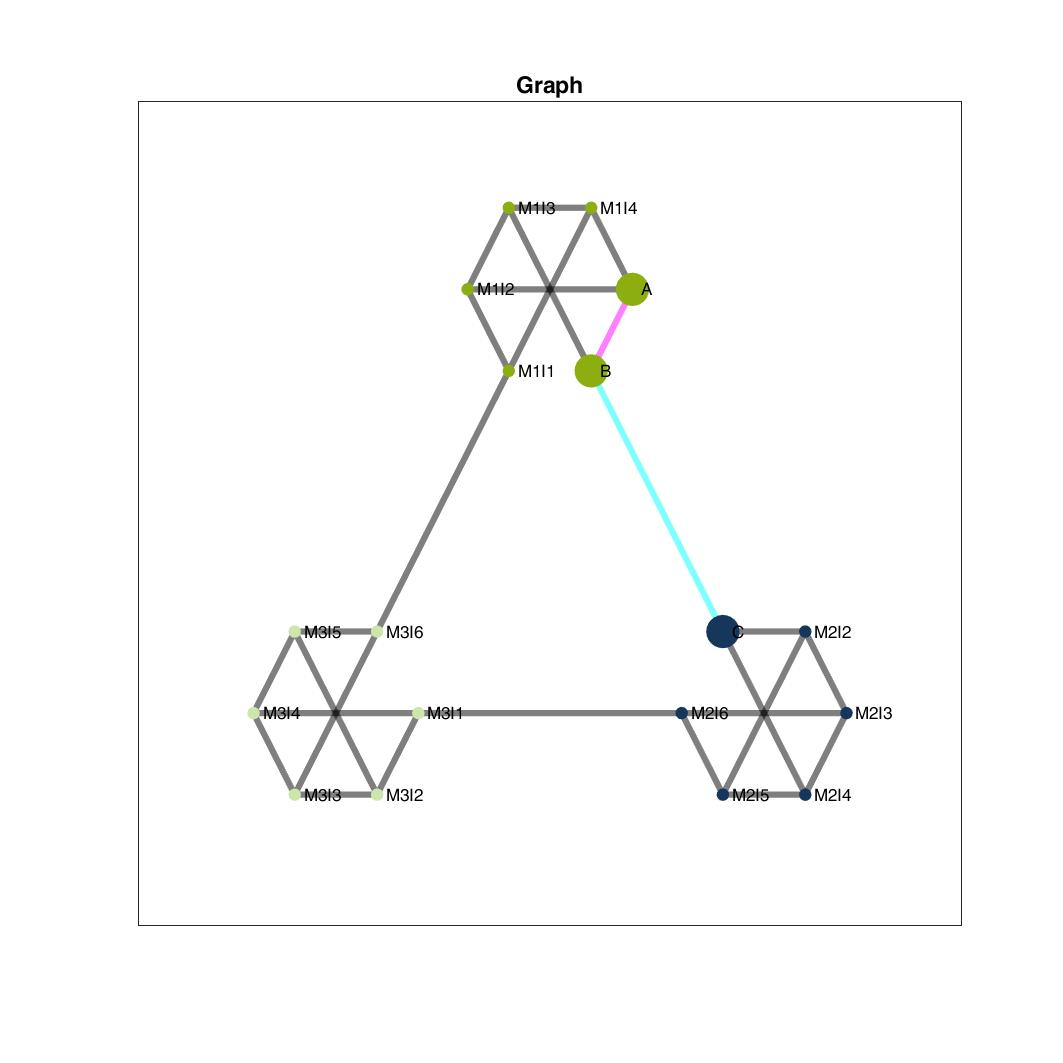
\includegraphics[width=85mm]{cat04_2716_tripletVisual.jpg}
    \caption{Beispielhafte Graphenstruktur für Kategorie 4}
    \label{fig:my_label}
\end{figure}


Aus der Anzahl der richtig identifizierten Stimuli für diese Kategorien wurde eine Trefferquote errechnet. Anschließend wurde diese für alle Teilnehmenden gemittelt und mittels \textit{t}-Test mit der Ratewahrscheinlichkeit verglichen. Bei drei Auswahlmöglichkeiten kann davon ausgegangen werden, dass die Wahrscheinlichkeit, durch Raten den richtigen Stimulus zu identifizieren, 1/3 beträgt.
Für Kategorie 1 und 5 war nicht eindeutig, welcher Stimulus als nicht/weniger zugehörig auszuwählen war. In Kategorie 1 gehörten alle Stimuli derselben Community an, der mittlere Stimulus war mit den anderen beiden direkt verbunden. Die äußeren Stimuli waren miteinander nur über zwei Schritte verbunden, daher sollte einer von beiden ausgewählt werden, nicht aber der mittlere.

\todo{Kategorie 5.1 fehlt!}

\paragraph{Sorting}
Für den zweiten Teil des Retrievals wurde für jeden ProbandInnen die Distanz errechnet, die zwischen den von ihm/ihr angeordneten Stimuli lag.
Auch für den zweiten Teil des Retrievals fand die Auswertung zunächst für jeden einzelnen Teilnehmenden statt, danach wurde ein Gruppendurchschnitt errechnet. Zunächst wurde die Distanz zwischen den von den ProbandInnen angeordneten Stimuli untereinander berechnet. Daraufhin wurde die Zugehörigkeit jedes Stimulus zu seiner Community bestimmt. Dadurch konnte die durchschnittliche Distanz berechnet werden zwischen Objekten innerhalb einer Community und der Distanz zu Stimuli, die einer anderen Community zugewiesen worden waren. Abschließend wurde mit einem gepaarten \textit{t}-Test überprüft, ob sich die durchschnittliche Distanz innerhalb von der Distanz außerhalb einer Community signifikant unterscheidet. Dabei wurde zwischen der Tag- und der Schlafbedingung unterschieden.

\subsection{Spezifische Hypothesen}

\paragraph{Hypothese 1 – Implizites Lernen der Struktur}
Die erste Hypothese lautete, dass die ProbandInnen die implizite Community-Struktur lernen.
Die Hypothese sollte als bestätigt gewertet werden, wenn beim \textit{Odd-one-out} der (laut Tabelle) richtige Stimulus signifikant häufiger ausgewhält wurde als die anderen. Beim \textit{Sorting} sollten die Stimuli einer Community einen geringeren Abstand untereinander haben als zu Stimuli einer anderen Community.

\textcolor{purple}{Triplet-Kategorien:
1) Triplets alle in einer Community: 1+2 (wird der Unterschied innerhalb einer Community durch zeitliche Nähe erkannt?)
2) Triplets 2 Stimuli aus einer Community, 1 Außenseiter: 3+4 (kann ein Stimulus von außerhalb identifiziert werden?)
2) Triplets zwischen den Communities: 5+6 (geschieht das Lernen aufgrund von zeitlicher Näher oder durch Community-Zugehörigkeit? Ist 6 signifikant, lernen wir durch zeitliche Nähe)
F-Test gegen 1/3 (Zufallswahrscheinlichkeit)}

Sorting:
t-Test (gepaart) innerhalb der Communities vs außerhalb
Voraussetzung: normalverteilt gegeben, da n>30 da keine Trennung nach Gruppen

\paragraph{Hypothese 2 – ProbandInnen zeigen Interferenz}
Laut Hypothese 2 sollten die ProbandInnen aus den nacheinander präsentierten Stimuli Schlüsse über die Beziehung von Stimuli ziehen können, die nicht direkt nacheinander gezeigt wurden. Objekte einer Community, die keine direkte Verbindung miteinander hatten, sollten also trotzdem als zueinander ähnlicher empfunden werden, als zu Objekten andere Communities.
Daher sollten in Kategorie 3 und 5 des \textit{Odd-one-out} diejenigen Stimuli gewählt werden, die zwar eine direkte Verbindung zum mittleren Stimulus hatten, jedoch zu einer anderen Community gehörten.

\textcolor{purple}{Triplet-Kategorien:
1) Triplets 2 Stimuli aus einer Community, 1 Außenseiter: 3+5 (kann ein Stimulus von außerhalb identifiziert werden?) \paragraph{Hypothese 2.2 – ProbandInnen in Schlafbedingung encodieren/konsolidieren besser} Triplet-Kategorien: Die Rate der richtig aussortierten Stimuli ist höher als für die ProbandInnen der Tagbedingung t-Test (gerichtet) Schlaf > Tag Sorting:außerhalb vs innerhalb getrennt für beide Gruppen}

\paragraph{Hypothese 3 – Einfluss von Schlaf}
Es wurde weiterhin davon ausgegangen, dass Schlaf einen positiven Einfluss auf die Konsolidierung der Graphenstruktur hat. Daher wurde hypothetisiert, dass ProbandInnen der Schlaf-Schlafbedingung bei beiden Teilen des \textit{Retrievals} signifikant bessere Ergebnisse erzielen als die der Taggruppe.

\section{Ergebnisse}
\label{S:3}
Bei der Datenauswertung wurden drei ProbandInnen ausgeschlossen. Grund dafür waren technische Probleme, Probleme mit dem Verständnis der zweiten Aufgabe sowie mangelnde Konzentration im ersten Teil.
Ein(e) weitere StudienteilnehmerIn wurde nicht in die statistische Analyse aufgenommen, da in der Sorting-Aufgabe lediglich ein Item bewegt wurde. Damit wurde die Aufgabe als nicht ausreichend bearbeitet angesehen.

\textcolor{purple}{Annahmen zu Varianz und Normalverteilung? Ja, dahin!}

\subsection{Wichtigste Befunde}
\paragraph{Odd-one-out}
Die durchschnittliche Trefferquote im ersten Teil des Retrievals, Odd-one-out, für die jeweiligen Kategorien kann der Tabelle \textcolor{purple}{X} entnommen werden. \textcolor{blue}{what about SD?}. Für Kategorie sechs wurde über alle ProbandInnen gemittelt eine höhere Trefferquote erzielt (\textit{M =} 36.2\%).
Der gerichtete \textit{t}-Test ergab, dass die Anzahl der richtig identifizierten Stimuli im Vergleich zur Ratewahrscheinlichkeit nicht signifikant höher war. Dies zeigte sich über alle analysierten Kategorien hinweg. \textcolor{purple}{(s. Tabelle oben)}
\todo{Hatten wir hier schon zwischen Gruppen getrennt was analysiert?}
\todo{Was ist mit EFFEKTSTÄRKEN??}

\begin{table}[h]
\centering
\begin{tabular}{l c c} %%l,c,r für Ausrichtung des Textes (links, mittig,rechts)
\hline
\textbf{Kategorie} & \textbf{Trefferquote} & \textbf{p-Wert}\\
\hline
2 & 32.1 & 0.723\\
3 & 33.5 & 0.471\\
4 & 33.6 & 0.433\\
6 & 36.2 & 0.163\\
8 & 33.6 & 0.436\\
\hline
\end{tabular}
\caption{Note. Trefferquote in Prozent}
\end{table}

\paragraph{Sorting}
Die durchschnittliche Distanz und Standardabweichung zwischen den angeordneten Stimuli innerhalb einer Gruppe sowie die Distanz zu den Objekten einer anderen Community lässt sich aus Tabelle \textcolor{purple}{X} entnehmen. Dabei wird unterschieden zwischen ProbandInnen, die der Tag- bzw. Nacht-Bedingung zugewiesen worden waren. Der gepaarte \textit{t}-Test ergab für die Schlafgruppe \textcolor{purple}{hier die Ergebnisse} und für die Taggruppe \textcolor{purple}{Ergebnisse}.

\begin{table}[h]
\centering
\captionsetup{justification=centering, margin = 1cm}
\begin{tabular}{l c c c c} %%l,c,r für Ausrichtung des Textes (links, mittig,rechts)
\hline
\textbf{Community} & \multicolumn{2}{c}{\textbf{Tag}} &  \multicolumn{2}{c}{\textbf{Schlaf}}\\
& Distanz & \textit{SD} & Distanz & \textit{SD} \\
\hline
Same & 0.43 & 0.09 & 0.43 & 0.12\\
Diff & 0.42 & 0.09 & 0.42 & 0.12\\
\hline
\end{tabular}
\caption{Note. Same = Same Community, Diff = Different Community}
\end{table}


\subsection{Bezug zur Fragestellung}
Hypothese 1 wurde ubjj j
Hypothese 2 konnte nljlk

\subsection{Auswertung}

\section{Diskussion}
\label{S:4}
\subsection{Ergebniszusammenfassung}


\subsection{Interpretation der Ergebnisse}

\subsection{Integration in die gegenwärtige Befundlage}

\subsection{Implikationen}

\subsection{Alternative Interpretationen}

The author names and affiliations could be formatted in two ways:
\begin{enumerate}[(1)]
\item Group the authors per affiliation.
\item Use footnotes to indicate the affiliations.
\end{enumerate}
See the front matter of this document for examples. You are recommended to conform your choice to the journal you are submitting to.

\subsection{Limitationen}
Stichprobenumfang war nicht ausreichend groß, bei der Unterteilung in beide Gruppen sank die jeweilige Gruppenzahl auf unter n=30, dadurch konnte nicht mehr von einer Normalverteilung ausgegangen werden. Auch durch die kurze Rekrutierungszeit bedingt. Weiteres Problem waren die zwei Zeitpunkte, zu denen die ProbandInnen Zeit für die Studienteilnahme haben mussten.
Vermutlich ziemlich homogene Stichprobe aufgrund der Rekrutierung im näheren Umkreis der Studiendurchführenden.
Frage nach externaler Validität.
Durchführungsobjektivität nicht ausreichend gegeben, da es nicht ausreichend standardisierte Anweisungen für die TestleiterInnen gab und die Testung an verschiedenen Orten stattfand. Störvariablen durch die Umwelt sind also nicht auszuschließen, und könnten vor allem die Konzentration der Teilnehmenden beeinflusst haben. Idealerweise hätten alle Testungen im selben Raum stattfinden sollen.
Auch technisch einige Probleme, da verschiedene Betriebssysteme verwendet wurden, die unterschiedlich zuverlässig funktionierten. (Deswegen musste(n) X Proband(en) ausgeschlossen werden).
Fragebogen zur Beurteilung der Schlafqualität sowie der Belastung am Tag war nicht standardisiert genug (offenes Antwortformat), wodurch die Auswertung erschwert wurde.
Wahl der sog. Marsobjekte könnte die Ergebnisse auch negativ beeinflusst haben. Viele ProbandInnen (die Mehrheit) gaben an, dass sie die Objekte nicht schön oder verwirrend fänden (NOCHMAL WORTLAUTE NACHGUCKEN). Ursprünglich wurden sie ausgewählt, um semantische Assoziationen auszuschließen. Es scheint fraglich, ob dies gelungen ist, da beim \textit{Sorting} teils sortiert wurde nach beispielsweise "Flug- und Erdobjekten". Entweder sollte man wieder Alltagsobjekte, die leicht zugänglich sind, wählen wie in Studie X (UNSERE), oder vielleicht noch abstraktere Objekte wie z.B. geometrische Formen.
Da die Studie im Rahmen eines universitären Seminars durchgeführt wurde, fehlten die finanziellen Mittel, um auf neurologische Grundlagen/Veränderungen zu testen.

\subsection{Ausblick}
[114, 135]
Pace-Schott EF, Milad MR, Orr SP, Rauch SL, Stickgold R, Pitman RK. Sleep promotes generalization of extinction of conditioned fear. Sleep 2009;32: 19e26.
Kleim B, Wilhelm FH, Temp L, Margraf J, Wiederhold BK, Rasch B. Sleep enhances exposure therapy. Psychol Med; 2013:1e9.
Schlaf unmittelbar nach einer Psychotherapie könnte die Integration von neuen/funktionalen Erinnerungen verbessern/enhance sowie die Transformation von dysfunktionalen Gedanken.
[135] Kurze Siesta-Perioden unmittelbar nach Expositions-Therapien führten zu einem signifikanten Rückgang von Angst bei PatientInnen mit Spinnen-Phobie.


\cite{Test}

\newpage

%\section{Literaturverzeichnis}
\bibliography{ref}

\clearpage

\appendix



\begin{table}[h]
\centering
\captionsetup{justification=centering, margin = 1cm}
\begin{tabular}{l c c c c c c c c}
\hline
\textbf{Kategorie} & \multicolumn{3}{c}{\textbf{Community}} &  \multicolumn{3}{c}{\textbf{Distanz}} & \textbf{Anz. Trials} & \textbf{Vorh.}\\
& A & B & C & AB & BC & AC \\
\hline
1 & 1 & 1 & 1 & 1 & 1 & 3 & 18 & not B\\
2 & 1 & 1 & 1 & 1 & 2 & 3 & 12 & C\\
3 & 1 & 1 & 2 & 2 & 2 & 2 & 6 & C\\
4 & 1 & 1 & 2 & 1 & 2 & 1 & 12 & C\\
5 & 1 & 1 & 2 & 3 & 4 & 1 & 6 & not A\\
6 & 1 & 2 & 3 & 1 & 4 & 5 & 6 & C\\
7 & 1 & 2 & 3 & 4 & 4 & 4 & 18 & random\\
8 & 1 & 2 & 3 & 4 & 3 & 5 & 18 & A\\
\hline
\end{tabular}
\caption{Note. Anz. Trials = Anzahl der Durchgänge, Vorh. = Vorhersage, relevant für die Trefferquote}
\end{table}

\todo{BESCHREIBUNG DER TRIPLETS NOCH REIN?}

\paragraph{Stimulus-Set}
\captionsetup[subfigure]{labelformat=empty}
\begin{figure}
\begin{subfigure}{0.2\textwidth}
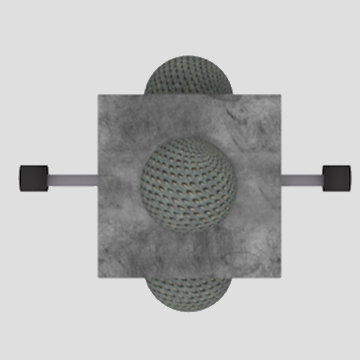
\includegraphics[width=\linewidth]{Bilder/Objekt1A.png}
\caption{Obj. 1, original} \label{fig:c}
\end{subfigure}\hspace{.5cm} %
\begin{subfigure}{0.2\textwidth}
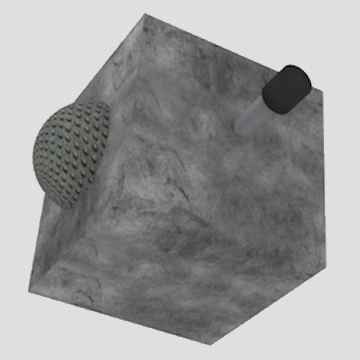
\includegraphics[width=\linewidth]{Bilder/Objekt1B.png}
\caption{Obj. 1, rotiert} \label{fig:d}
\end{subfigure} \hspace{.5cm}%
\begin{subfigure}{0.2\textwidth}
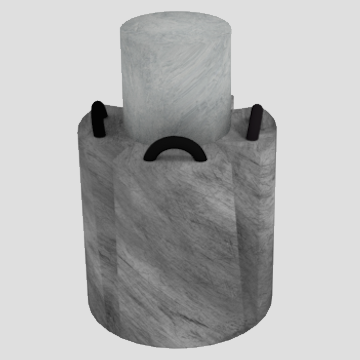
\includegraphics[width=\linewidth]{Bilder/Objekt2A.png}
\caption{Obj. 2, original} \label{fig:e}
\end{subfigure}\hspace{.5cm}
\begin{subfigure}{0.2\textwidth}
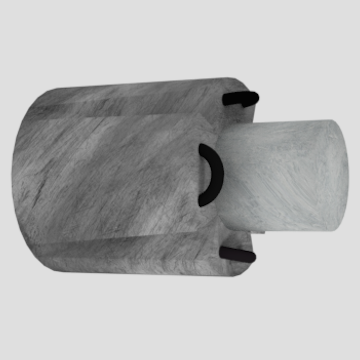
\includegraphics[width=\linewidth]{Bilder/Objekt2B.png}
\caption{Obj. 2, rotiert} \label{fig:f}
\end{subfigure}\hspace{.5cm}

\medskip
\begin{subfigure}{0.2\textwidth}
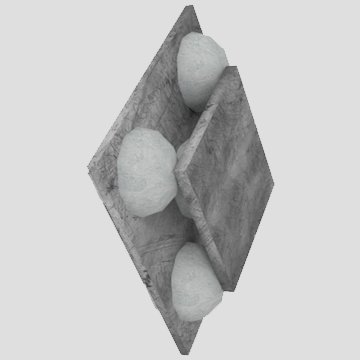
\includegraphics[width=\linewidth]{Bilder/Objekt3A.png}
\caption{Obj. 3, original} \label{fig:c}
\end{subfigure}\hspace{.5cm} %
\begin{subfigure}{0.2\textwidth}
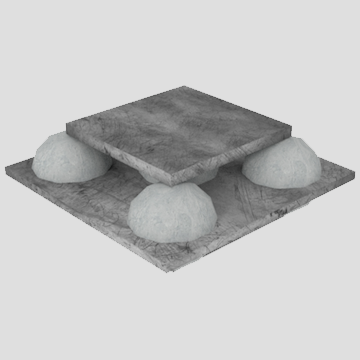
\includegraphics[width=\linewidth]{Bilder/Objekt3B.png}
\caption{Obj. 3, rotiert} \label{fig:d}
\end{subfigure} \hspace{.5cm}%
\begin{subfigure}{0.2\textwidth}
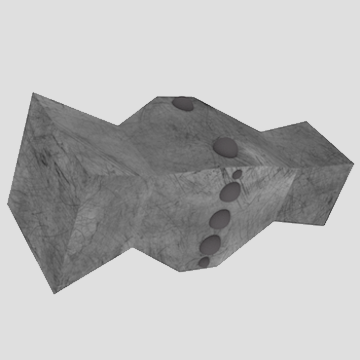
\includegraphics[width=\linewidth]{Bilder/Objekt4A.png}
\caption{Obj. 4, original} \label{fig:e}
\end{subfigure}\hspace{.5cm}
\begin{subfigure}{0.2\textwidth}
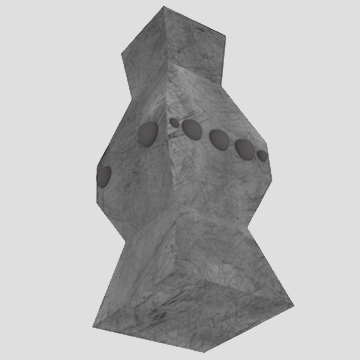
\includegraphics[width=\linewidth]{Bilder/Objekt4B.png}
\caption{Obj. 4, rotiert} \label{fig:f}
\end{subfigure}\hspace{.5cm}

\medskip
\begin{subfigure}{0.2\textwidth}
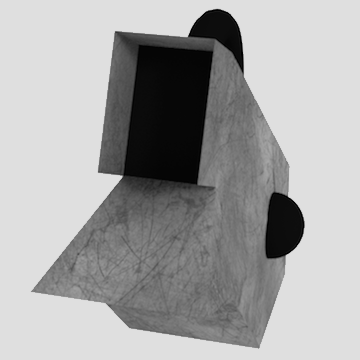
\includegraphics[width=\linewidth]{Bilder/Objekt5A.png}
\caption{Obj. 5, original} \label{fig:c}
\end{subfigure}\hspace{.5cm} %
\begin{subfigure}{0.2\textwidth}
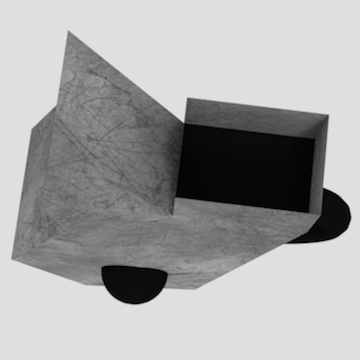
\includegraphics[width=\linewidth]{Bilder/Objekt5B.png}
\caption{Obj. 5, rotiert} \label{fig:d}
\end{subfigure} \hspace{.5cm}%
\begin{subfigure}{0.2\textwidth}
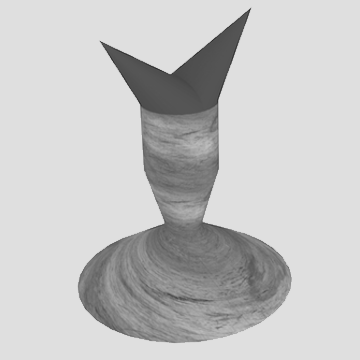
\includegraphics[width=\linewidth]{Bilder/Objekt6A.png}
\caption{Obj. 6, original} \label{fig:e}
\end{subfigure}\hspace{.5cm}
\begin{subfigure}{0.2\textwidth}
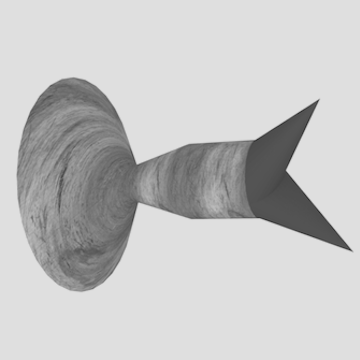
\includegraphics[width=\linewidth]{Bilder/Objekt6B.png}
\caption{Obj. 6, rotiert} \label{fig:f}
\end{subfigure}\hspace{.5cm}

\medskip
\begin{subfigure}{0.2\textwidth}
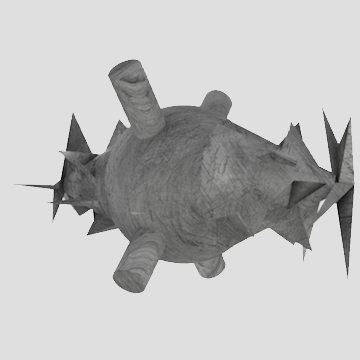
\includegraphics[width=\linewidth]{Bilder/Objekt7A.png}
\caption{Obj. 7, original} \label{fig:c}
\end{subfigure}\hspace{.5cm} %
\begin{subfigure}{0.2\textwidth}
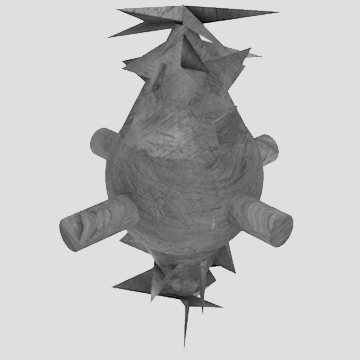
\includegraphics[width=\linewidth]{Bilder/Objekt7B.png}
\caption{Obj. 7, rotiert} \label{fig:d}
\end{subfigure} \hspace{.5cm}%
\begin{subfigure}{0.2\textwidth}
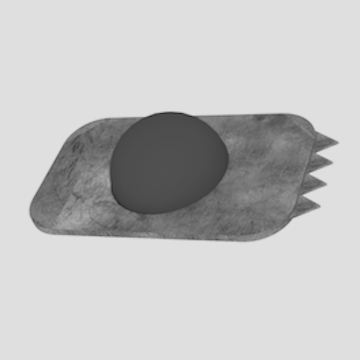
\includegraphics[width=\linewidth]{Bilder/Objekt8A.png}
\caption{Obj. 8, original} \label{fig:e}
\end{subfigure}\hspace{.5cm}
\begin{subfigure}{0.2\textwidth}
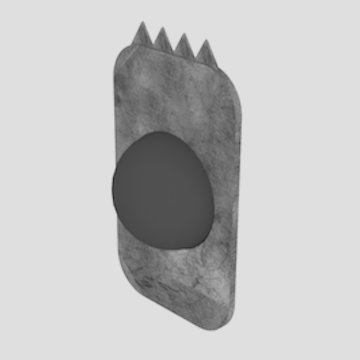
\includegraphics[width=\linewidth]{Bilder/Objekt8B.png}
\caption{Obj. 8, rotiert} \label{fig:f}
\end{subfigure}\hspace{.5cm}

\medskip
\begin{subfigure}{0.2\textwidth}
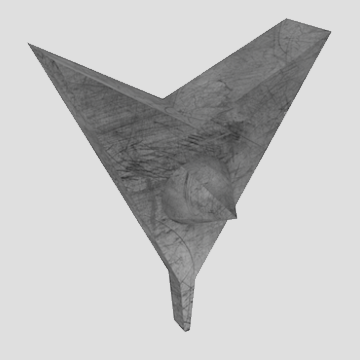
\includegraphics[width=\linewidth]{Bilder/Objekt9A.png}
\caption{Obj. 9, original} \label{fig:c}
\end{subfigure}\hspace{.5cm} %
\begin{subfigure}{0.2\textwidth}
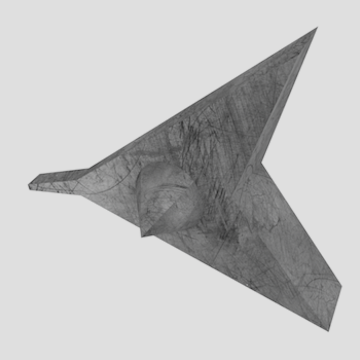
\includegraphics[width=\linewidth]{Bilder/Objekt9B.png}
\caption{Obj. 9, rotiert} \label{fig:d}
\end{subfigure} \hspace{.5cm}%
\begin{subfigure}{0.2\textwidth}
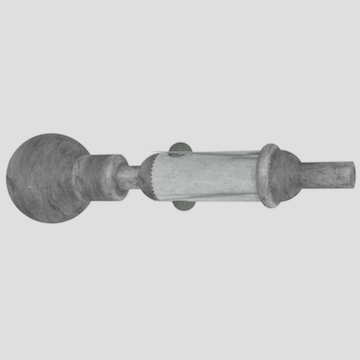
\includegraphics[width=\linewidth]{Bilder/Objekt10A.png}
\caption{Obj. 10, original} \label{fig:e}
\end{subfigure}\hspace{.5cm}
\begin{subfigure}{0.2\textwidth}
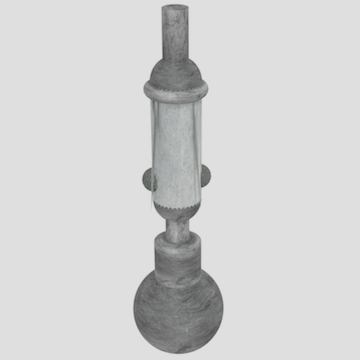
\includegraphics[width=\linewidth]{Bilder/Objekt10B.png}
\caption{Obj. 10, rotiert} \label{fig:f}
\end{subfigure}\hspace{.5cm}

\medskip
\begin{subfigure}{0.2\textwidth}
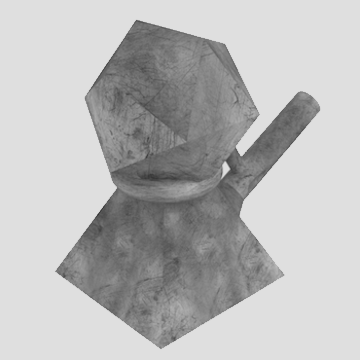
\includegraphics[width=\linewidth]{Bilder/Objekt11A.png}
\caption{Obj. 11, original} \label{fig:c}
\end{subfigure}\hspace{.5cm} %
\begin{subfigure}{0.2\textwidth}
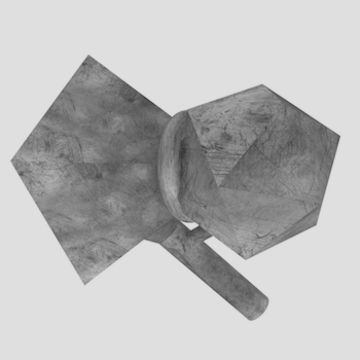
\includegraphics[width=\linewidth]{Bilder/Objekt11B.png}
\caption{Obj. 11, rotiert} \label{fig:d}
\end{subfigure} \hspace{.5cm}%
\begin{subfigure}{0.2\textwidth}
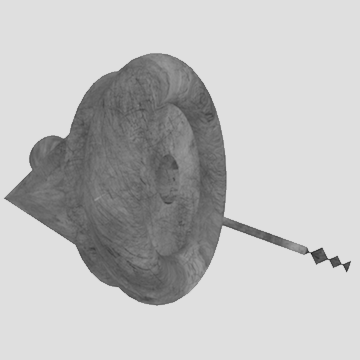
\includegraphics[width=\linewidth]{Bilder/Objekt12A.png}
\caption{Obj. 12, original} \label{fig:e}
\end{subfigure}\hspace{.5cm}
\begin{subfigure}{0.2\textwidth}
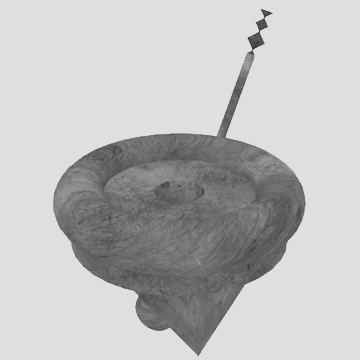
\includegraphics[width=\linewidth]{Bilder/Objekt12B.png}
\caption{Obj. 12, rotiert} \label{fig:f}
\end{subfigure}\hspace{.5cm}

\medskip
\begin{subfigure}{0.2\textwidth}
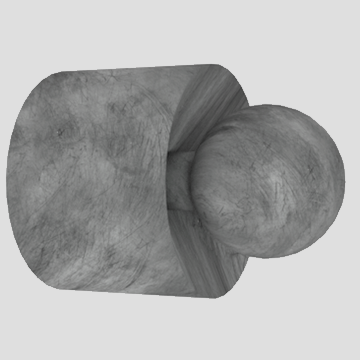
\includegraphics[width=\linewidth]{Bilder/Objekt13A.png}
\caption{Obj. 13, original} \label{fig:c}
\end{subfigure}\hspace{.5cm} %
\begin{subfigure}{0.2\textwidth}
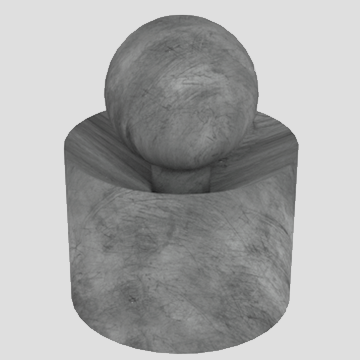
\includegraphics[width=\linewidth]{Bilder/Objekt13B.png}
\caption{Obj. 13, rotiert} \label{fig:d}
\end{subfigure} \hspace{.5cm}%
\begin{subfigure}{0.2\textwidth}
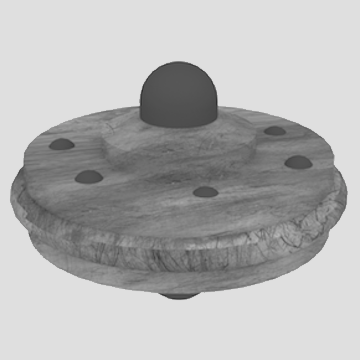
\includegraphics[width=\linewidth]{Bilder/Objekt14A.png}
\caption{Obj. 14, original} \label{fig:e}
\end{subfigure}\hspace{.5cm}
\begin{subfigure}{0.2\textwidth}
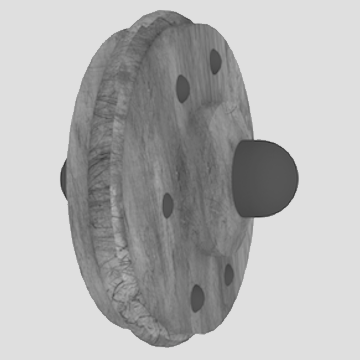
\includegraphics[width=\linewidth]{Bilder/Objekt14B.png}
\caption{Obj. 14, rotiert} \label{fig:f}
\end{subfigure}\hspace{.5cm}

\medskip
\begin{subfigure}{0.2\textwidth}
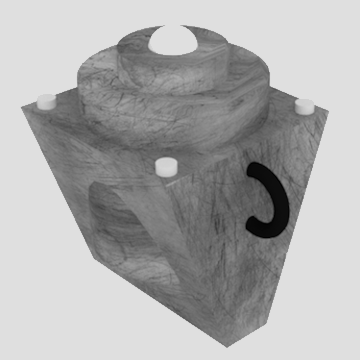
\includegraphics[width=\linewidth]{Bilder/Objekt15A.png}
\caption{Obj. 15, original} \label{fig:c}
\end{subfigure}\hspace{.5cm} %
\begin{subfigure}{0.2\textwidth}
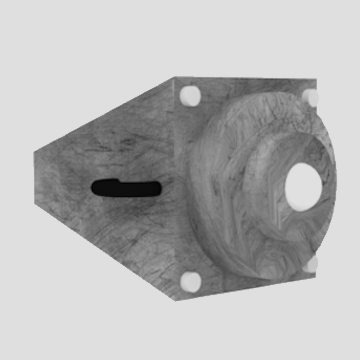
\includegraphics[width=\linewidth]{Bilder/Objekt15B.png}
\caption{Obj. 15, rotiert} \label{fig:d}
\end{subfigure} \hspace{.5cm}%
\begin{subfigure}{0.2\textwidth}
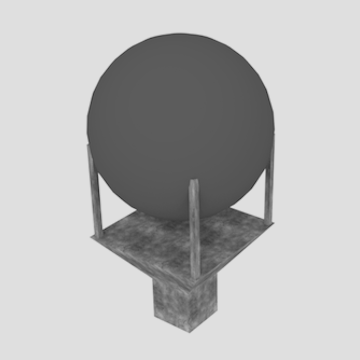
\includegraphics[width=\linewidth]{Bilder/Objekt16A.png}
\caption{Obj. 16, original} \label{fig:e}
\end{subfigure}\hspace{.5cm}
\begin{subfigure}{0.2\textwidth}
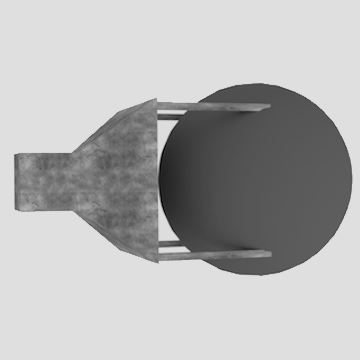
\includegraphics[width=\linewidth]{Bilder/Objekt16B.png}
\caption{Obj. 16, rotiert} \label{fig:f}
\end{subfigure}\hspace{.5cm}

\medskip
\begin{subfigure}{0.2\textwidth}
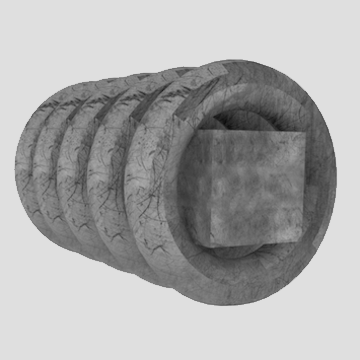
\includegraphics[width=\linewidth]{Bilder/Objekt17A.png}
\caption{Obj. 17, original} \label{fig:c}
\end{subfigure}\hspace{.5cm} %
\begin{subfigure}{0.2\textwidth}
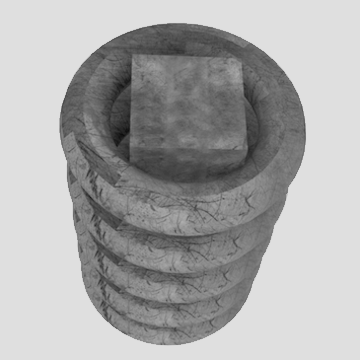
\includegraphics[width=\linewidth]{Bilder/Objekt17B.png}
\caption{Obj. 17, rotiert} \label{fig:d}
\end{subfigure} \hspace{.5cm}%
\begin{subfigure}{0.2\textwidth}
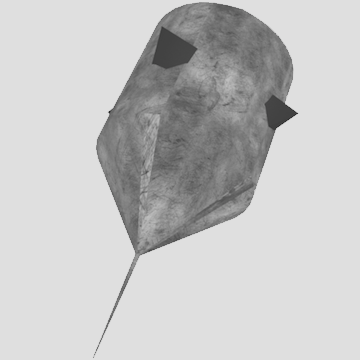
\includegraphics[width=\linewidth]{Bilder/Objekt18A.png}
\caption{Obj. 18, original} \label{fig:e}
\end{subfigure}\hspace{.5cm}
\begin{subfigure}{0.2\textwidth}
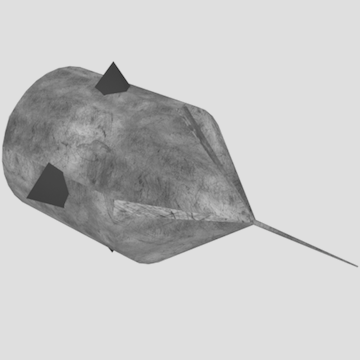
\includegraphics[width=\linewidth]{Bilder/Objekt18B.png}
\caption{Obj. 18, rotiert} \label{fig:f}
\end{subfigure}\hspace{.5cm}

\caption{My complicated figure} \label{fig:1}
\end{figure}



\end{document}
